\documentclass[titlepage]{jarticle}
\usepackage[dvipdfmx]{graphicx}
\usepackage{listings}
\usepackage{here}
\usepackage{r04ec-exp}

%
\lstset{
  basicstyle={\ttfamily},
  identifierstyle={\small},
  commentstyle={\smallitshape},
  keywordstyle={\small\bfseries},
  ndkeywordstyle={\small},
  stringstyle={\small\ttfamily},
  frame={tb},
  breaklines=true,
  columns=[l]{fullflexible},
  numbers=left,
  xrightmargin=0zw,
  xleftmargin=3zw,
  numberstyle={\scriptsize},
  stepnumber=1,
  numbersep=1zw,
  lineskip=-0.5ex,
  language=c
}
\renewcommand{\lstlistingname}{ソースコード}
\makeatletter
\newcommand{\figcaption}[1]{\def\@captype{figure}\caption{#1}}
\newcommand{\tblcaption}[1]{\def\@captype{table}\caption{#1}}
\makeatother
%%% 表紙の記載事項設定
%
% 実験題目  ※レポートを書くときは,まず,タイトルを正しいものに変えましょう
%
\title{信号処理プログラミングl}
% 学年・番号
\grade{4年37番}%
% 氏名
\author{本間 三暉}
% 班(後期は班に分かれて実験をする.そのときは,ここに班番号を記入する.)
\team{}
% 提出日
\date{2022年5月20日}
% 実験日
\expdate{2022年4月14日,4月21日,4月28日,5月19日}
% 共同実験者
% グループに分かれて実験をするテーマでは,グループメンバーの番号名前を書く.
\coauthor{%
}
%
%記載例:
%\coauthor{%
%  2番 & 新潟 花子\\
%  11番 & 三条 次郎}
%%
\begin{document}
\maketitle

\section{目的}
アナログ信号をディジタルデータに変換し,ディジタル機器で処理するために必要な基礎事項について学習し,C言語で基本的な信号処理プログラムを作成する.また,実用的な音声フォーマットの一つであるWAVEファイルの構造を理解し,音声データの出入力プログラムを作成する.
\section{演習}
今回の実験の演習では,特に明言されていない限りソースコード\ref{include}に示すヘッダファイル,及びソースコード\ref{define}に示す定義ファイルが読み込まれているものとする.なお,pi.hは付録Bのリスト6である.
\begin{lstlisting}[caption=ヘッダファイル,label=include]
#include <stdio.h>
#include <stdlib.h>
#include <math.h>
#include <string.h>
#include <time.h>
#include <ctype.h>

#include "pi.h"
  \end{lstlisting}
\begin{lstlisting}[caption=定義ファイル,label=define]
#define BUFSIZE 80
#define A_BIAS 0x80
#define DATANUM 101 
  \end{lstlisting}

また,それ以前の演習で示した自作関数はそれ以降のソースコードで断りなく使用する.
\subsection{次の指示に従いプログラムを作成し,出力をgnuplotで可視化して動作確認を行え.}
\subsubsection{任意の弧度rを[$0:2\pi$]の範囲内に収まるように変換する関数radを作成せよ.}
ソースコード\ref{rad}に関数radを示す.
\begin{lstlisting}[caption=double rad(double r),label=rad]
    double mod;
    mod = fmod(r,2 * PI);
    if(r < 0) mod = mod + 2 * PI;
    return mod;
   \end{lstlisting}

数学関数fmodはrが負の場合[$-2\pi:0$]の値を取る.
このままでは目的の値は得られないので,rが負の場合はfmodが返した値に$2\pi$[rad]を加えることで値を[$0:2\pi$]の範囲に収める事ができる.

これを出力すると図\ref{fig:rad}となる.

\subsubsection{任意の弧度rに対して,のこぎり波の振幅値を求める関数sawを作成せよ.}
ソースコード\ref{saw}に関数sawを示す.
\begin{lstlisting}[caption=double saw(double r),label=saw]
    double saw_wave;
    saw_wave = 1 - rad(r) / PI;
    return saw_wave;
   \end{lstlisting}
ソースコード\ref{rad}のradにおいて出力値の変化幅は$2\pi$[rad]である.これに対してのこぎり波の変化幅は$2$[rad]であるので,関数radの戻り値を$\pi$で割ることによって変化幅を$2$[rad]にすることができる.
また理想的なのこぎり波の範囲は[$-1:1$]で,$0,2\pi,4\pi$で$-1$から$1$へ瞬時に変化するため,ソースコード\ref{saw}の2行目のように記述すれば良い.

これを出力すると図\ref{fig:saw}となる.
\begin{figure}[H]
  \begin{minipage}{0.495\hsize}
    \centering
    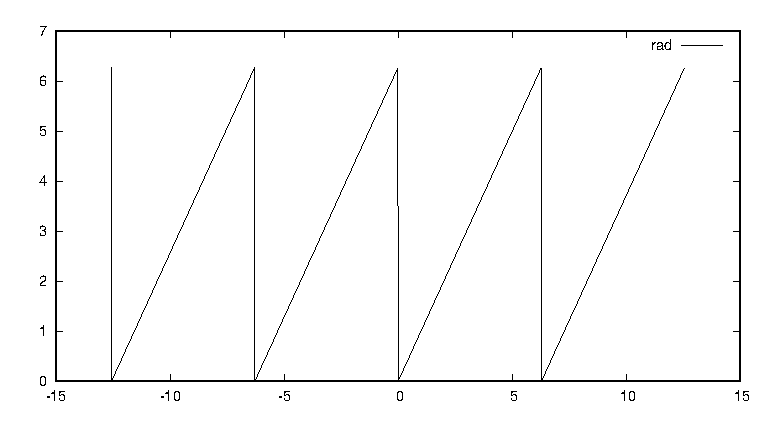
\includegraphics[width=7cm]{EPS/rad1.eps}
    \caption{radの出力波形}
    \label{fig:rad}
  \end{minipage}
  \begin{minipage}{0.495\hsize}
    \centering
    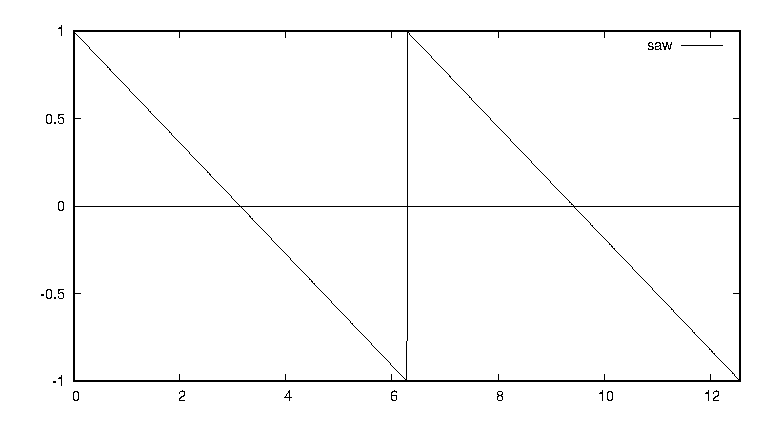
\includegraphics[width=7cm]{EPS/saw1.eps}
    \caption{sawの出力波形}
    \label{fig:saw}
  \end{minipage}
\end{figure}
\subsection{次の指示に従いプログラムを作成し,動作を確認せよ.}
\subsubsection{リスト2のコードを解析し,完成させよ.振幅 100,周波数 3[Hz]のデータをgnuplotでグラフ化し,サンプリングの効果を確認せよ.}
リスト2のコードを完成させたものをソースコード\ref{sin10af1.c}に示す.
\begin{lstlisting}[caption=リスト2変更部分のみ,label=sin10af1.c]
  for (t = 0; t <= T_END; t += DT) {
    rad = t * (frq / 1000) * 2 * PI;
    vin = amp * sin(rad) + A_BIAS;
    vout = vin;
    printf("%4d, %4d\n", t, vout);
  }
   \end{lstlisting}

これを出力すると\ref{sin100f3}となる.
\begin{figure}[H]
  \centering
  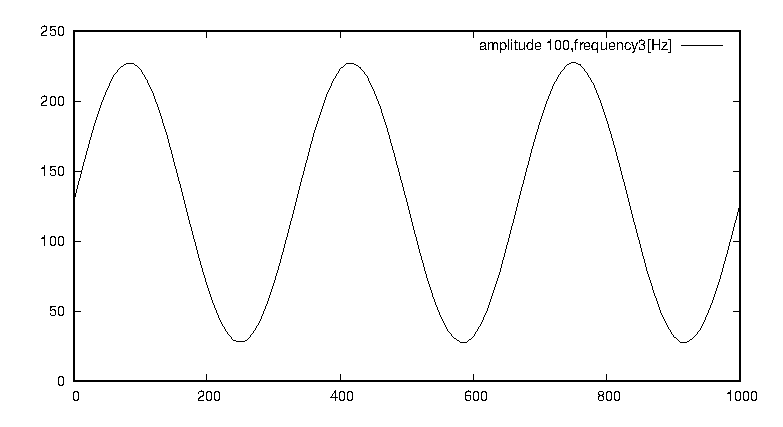
\includegraphics[width=7cm]{EPS/sin100f3.eps}
  \caption{振幅100,周波数3[Hz]}
  \label{sin100f3}
\end{figure}
\subsubsection{振幅 140,周波数 3[Hz]のデータを生成し,その波形を確認せよ.波形に不具合があれば,その原因を考えて不具合を軽減するような修正を行え.}
振幅 140,周波数 3[Hz]の条件で出力した波形は図\ref{sin140f3:before}となった.これはvoutがunsigned char型であり,[$0:225$]の範囲の値しか取らないため,この範囲に入らない値はオーバーフローしてしまい別の値として出力されてしまうためだと考えられる.

これを修正するために,範囲を超えてしまったものは範囲内の値に修正すれば良い.これを実装したものをソースコード\ref{sin140f3}に示す.
\begin{lstlisting}[caption=修正後,label=sin140f3]
  for (t = 0; t <= T_END; t += DT) {
    rad = t * (frq / 1000) * 2 * PI;
    vin = amp * sin(rad) + A_BIAS;
    if (vin < 0) vin = 0;
    if (vin > 255) vin = 255;
    vout = vin;
    printf("%4d, %4d\n", t, vout);
  }
   \end{lstlisting}

また,これを出力したものを図\ref{sin140f3:after}に示す.
\begin{figure}[H]
  \begin{minipage}{0.495\hsize}
    \centering
    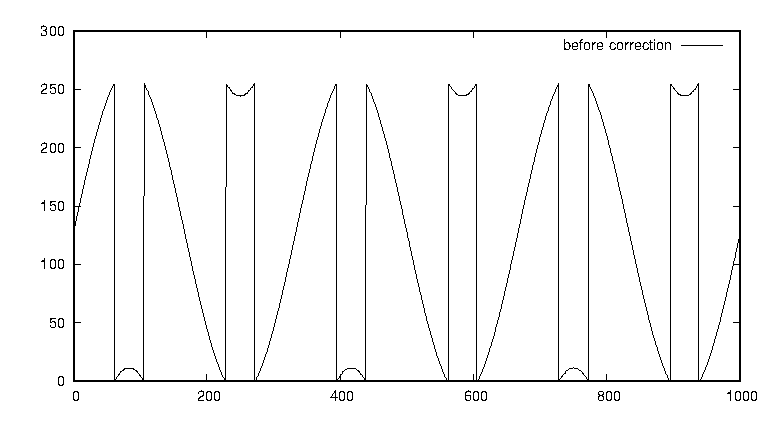
\includegraphics[width=7cm]{EPS/sin140f3_before.eps}
    \caption{振幅140,周波数3[Hz]修正前}
    \label{sin140f3:before}
  \end{minipage}
  \begin{minipage}{0.495\hsize}
    \centering
    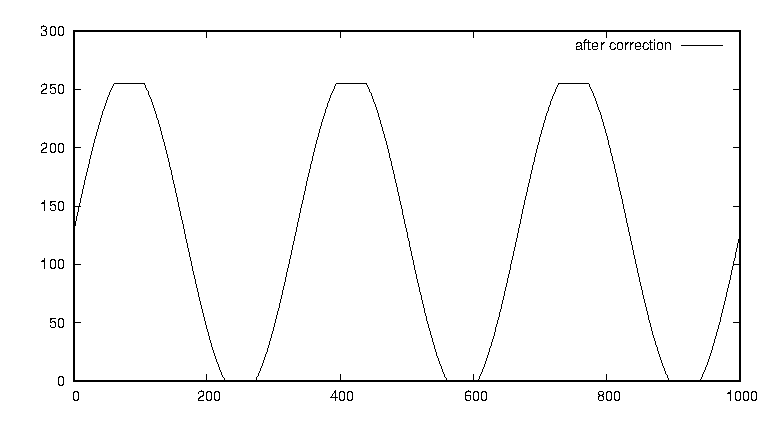
\includegraphics[width=7cm]{EPS/sin140f3_after.eps}
    \caption{振幅140,周波数3[Hz]修正後}
    \label{sin140f3:after}
  \end{minipage}
\end{figure}
\setcounter{subsubsection}{4}
\subsubsection{サンプリング定理を満たさないような高い周波数の正弦波をPCMによりディジタルデータ化すると,周波数や位相が全く異なる波のように見えることがある.この現象を実際に観測せよ.}

この現象をまとめたものを図\ref{PCM}に示す.なお,DTは標本化間隔のことである.
\begin{figure}[H]
  \centering
  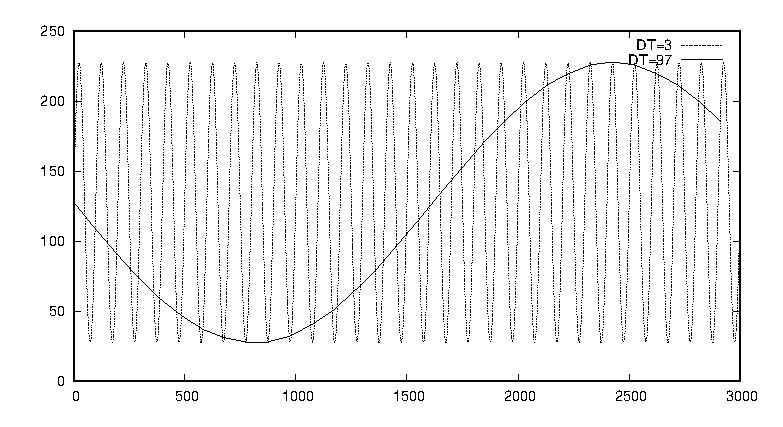
\includegraphics[width=7cm]{EPS/PCM.eps}
  \caption{振幅100,周波数10[Hz]}
  \label{PCM}
\end{figure}
このように同じ振幅同じ周波数のはずなのに,全く違う波形に見えてしまうことを観測した.この現象は高速回転するタイヤなどでも起きるものなのでかなり身近なものである.
\subsection{次のプログラムを作成して動作を確認せよ.出力の形式はプログラム例3を参考にして,加工後の振幅値を一列加えることにしておくと良い.}
\subsubsection{白色雑音を加えるオフライン型プログラムを作成せよ.}
白色雑音を加えるオフライン型プログラムをソースコード\ref{add-wn2.c}に示す.
\begin{lstlisting}[caption=add-wn2.c,label=add-wn2.c]
#define BUFSIZE 80
#define DATANUM 101
#define ROUND(x) ((x > 0) ? (x * 0.5) : (x - 0.5))

int main(int argc, char **argv) {
  int n, n_keep;
  int tm[DATANUM], amp[DATANUM], aout[DATANUM];
  int nmax;
  double err;
  char buf[BUFSIZE];
  FILE *fp;

  if (argc != 3) {
    fprintf(stderr, "Usage: %s infile max_noise\n", argv[0]);
    return EXIT_FAILURE;
  }
  if ((fp = fopen(argv[1], "r")) == NULL) {
    fprintf(stderr, "File: %s cannot open\n", argv[1]);
    return EXIT_FAILURE;
  }

  for (n = 0; n < DATANUM;) {
    if (fgets(buf, sizeof(buf), fp) == NULL) break;
    if (buf[0] == '#') {
      printf("%s", buf);
      continue;
    }
    tm[n] = atoi(strtok(buf, ","));
    amp[n] = atoi(strtok(NULL, "\r\n\0"));
    n++;
  }
  fclose(fp);

  n_keep = n;
  nmax = atoi(argv[2]);
  printf("# WN %d\n", nmax);
  srand((unsigned)time(NULL));
  for (n = 0; n < DATANUM; n++) {
    err = nmax * (2.0 * rand() / RAND_MAX - 1.0);
    aout[n] = amp[n] + ROUND(err);
    if (aout[n] < 0) aout[n] = 0;
    if (aout[n] > 255) aout[n] = 255;
  }
  for (n = 0; n < n_keep; n++) {
#if defined TEST
    printf("%4d, %4d, %4d\n", tm[n], amp[n], aout[n]);
#else
    printf("%4d,%4d\n", tm[n], aout[n]);
#endif
  }
  return EXIT_SUCCESS;
}
   \end{lstlisting}

ソースコード\ref{add-wn2.c}において22行目のfor文の条件式に n++ がなく30行目に n++ がある理由は,for文の条件式に n++ があると continue の処理をした際に n++ が実行されてしまい,出力用の配列に代入するのがうまくいかないからである.

振幅 100,周波数 3[Hz]の正弦波に最大振幅を10とした白色雑音を加えた波形と元の波形を重ねたものを図\ref{fig:white_noise}に示す.
\begin{figure}[H]
  \centering
  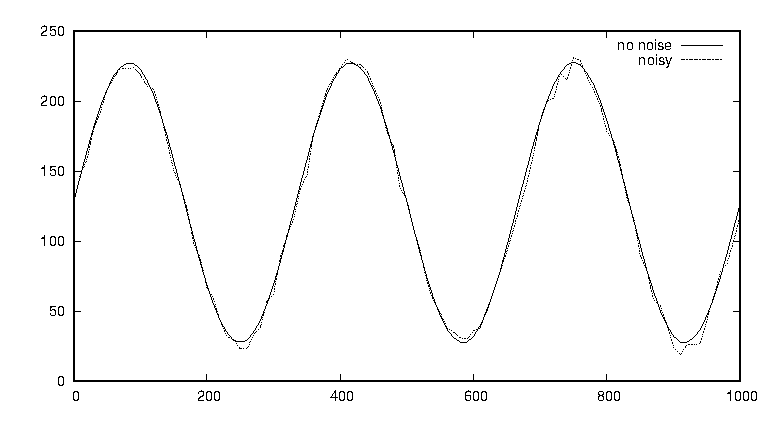
\includegraphics[width=7cm]{EPS/white_noise.eps}
  \caption{ノイズなしとノイズあり}
  \label{fig:white_noise}
\end{figure}
最大振幅をそこまで大きくしなかったが,目に見えるほどずれてしまっているので,本当にノイズを除去できるのか不安である.
\subsubsection{3点単純平均移動プログラムを作成せよ.}
オンライン型をソースコード\ref{mwave3-1.c},オフライン型をソースコード\ref{mwave3-2.c}に示す.
\begin{lstlisting}[caption=mwave3-1.c,label=mwave3-1.c]
#define MOVING_AVERAGE 3
int main(int argc, char **argv) {
  int tm,tm_1, ain, aout, nmax, n = 0;
  double err_3add = 0.0, err_2before, err_1before, now;
  char buf[BUFSIZE];
  FILE *fp;

  if (argc != 2) {
    fprintf(stderr, "Usage: %s infile max_noise\n", argv[0]);
    return EXIT_FAILURE;
  }
  if ((fp = fopen(argv[1], "r")) == NULL) {
    fprintf(stderr, "File: %s cannot open\n", argv[1]);
    return EXIT_FAILURE;
  }
  while (fgets(buf, sizeof(buf), fp) != NULL) {
    if (buf[0] == '#') {
      printf("%s", buf);
      continue;
    }
    tm = atoi(strtok(buf, ","));
    tm_1 = tm;
    ain = atoi(strtok(NULL, "\r\n\0"));
    err_2before = err_1before;
    err_1before = now;
    now = ain;
    err_3add += ain;
    if (n < MOVING_AVERAGE - 1) {
      n++;
      continue;
    }

    aout = err_3add / MOVING_AVERAGE;
    if (aout < 0) aout = 0;
    if (aout > 255) aout = 255;

#if defined TEST
    printf("%4d, %4d, %4d\n", tm_1, ain, aout);
#else
    printf("%4d,%4d\n", tm_1, aout);
#endif

    err_3add -= err_2before;

  }
  fclose(fp);
  return EXIT_SUCCESS;
}
   \end{lstlisting}
\begin{lstlisting}[caption=mwave3-2.c,label=mwave3-2.c]
int main(int argc, char **argv) {
  int n, i;
  int tm[DATANUM], amp[DATANUM], aout[DATANUM], editing[DATANUM - 1];

  int nmax;
  double err, err_3add = 0;
  char buf[BUFSIZE];
  FILE *fp;

  if (argc != 2) {
    fprintf(stderr, "Usage: %s infile max_noise\n", argv[0]);
    return EXIT_FAILURE;
  }
  if ((fp = fopen(argv[1], "r")) == NULL) {
    fprintf(stderr, "File: %s cannot open\n", argv[1]);
    return EXIT_FAILURE;
  }
  for (n = 0; n < DATANUM;) {
    if (fgets(buf, sizeof(buf), fp) == NULL) break;
    if (buf[0] == '#') {
      printf("%s", buf);
      continue;
    }
    tm[n] = atoi(strtok(buf, ","));
    amp[n] = atoi(strtok(NULL, "\r\n\0"));
    n++;
  }
  fclose(fp);
  for (n = 0; n < MOVING_AVERAGE / 2 + 1; n++) {
    err_3add += amp[n];
  }

  for (n = MOVING_AVERAGE / 2; n < DATANUM - 1; n++) {
    err_3add += amp[n + MOVING_AVERAGE / 2];
    aout[n] = err_3add / MOVING_AVERAGE;
    err_3add -= amp[n - MOVING_AVERAGE / 2];
    if (aout[n] < 0) aout[n] = 0;
    if (aout[n] > 255) aout[n] = 255;
  }
  for (n = 1; n < DATANUM; n++) {
#if defined TEST
    printf("%4d, %4d, %4d\n", tm[n], amp[n], aout[n]);
#else
    printf("%4d,%4d\n", tm[n], aout[n]);
#endif
  }
  return EXIT_SUCCESS;
}
   \end{lstlisting}

オンライン型が最新のデータから3つを保持するのに対し,オフライン型はすべてのデータが既知であるため配列をうまく活用して処理することが求められる.両方とも同じやり方で3点の平均値を求めているが上記のやり方が一番計算量が少ないと思われる.

雑音を含んだ波形を3点単純移動平均プログラムで復元したものと雑音を含んだ波形を図\ref{mvave3}に示す.また,復元したものともとの波形を図\ref{sin_mvave3}に示す.
\begin{figure}[H]
  \begin{minipage}{0.495\hsize}
    \centering
    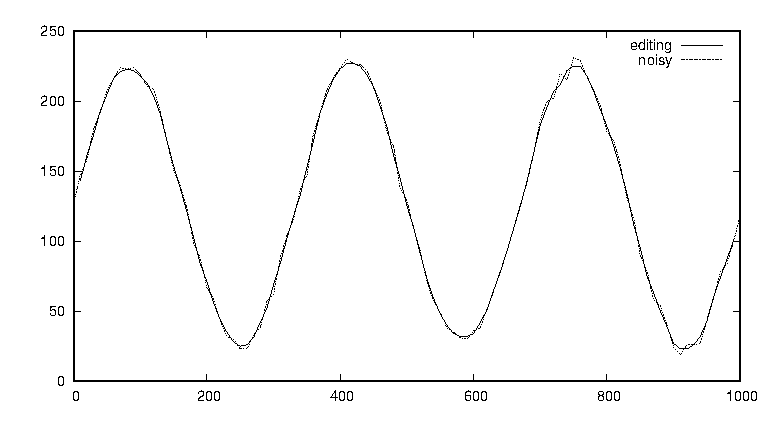
\includegraphics[width=7cm]{EPS/point_3_noise_deleat.eps}
    \caption{ノイズありとノイズ除去後}
    \label{mvave3}
  \end{minipage}
  \begin{minipage}{0.495\hsize}
    \centering
    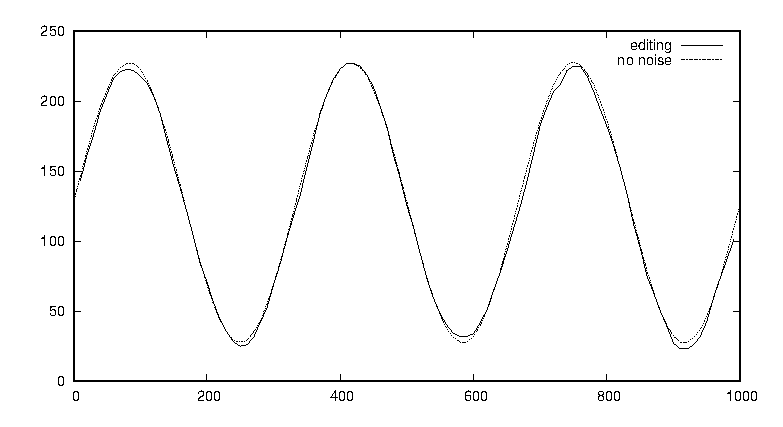
\includegraphics[width=7cm]{EPS/sin100f3_3point.eps}
    \caption{ノイズなしとノイズ除去後}
    \label{sin_mvave3}
  \end{minipage}
\end{figure}
この結果を見ると,やや大きくずれた部分は完全に雑音を取り去るのは難しそうであるが,概ねもとの波形に近づけることができていると考えられる.
\subsection{次の指示に従い,式変形及びプログラム作成と動作確認を行え.}
\subsubsection{式(7)を変形して式(8)を導出する過程を示せ.}
テキストの式(7)は以下の通りである.
\begin{eqnarray*}
  \sigma^{2} & = & \frac{1}{N} \sum_{i=1}^{N}(x_{i} - \bar{x})^{2}
\end{eqnarray*}

中身を展開してそれぞれの項に分解し,定数を前に出す.

\begin{eqnarray*}
  \sigma^{2} & = & \frac{1}{N} \sum_{i=1}^{N}(x_{i}) - \frac{2\bar{x}}{N} \sum_{i=1}^{N}x_{i}+\frac{1}{N} \sum_{i=1}^{N}\bar{x}^{2}
\end{eqnarray*}

このとき,

\begin{eqnarray*}
  \bar{x} & = & \frac{1}{N} \sum_{i=1}^{N}x_{i}
\end{eqnarray*}

なので,

\begin{eqnarray*}
  \sigma^{2} & = & \frac{1}{N} \sum_{i=1}^{N}(x_{i}) - 2\bar{x}^{2} + \bar{x}^{2}\\
  \sigma^{2} & = & \frac{1}{N} \sum_{i=1}^{N}(x_{i}) - \bar{x}^{2}
\end{eqnarray*}

これは式(8)であるので,式(7)を変形して式(8)を導出することができた.

\subsubsection{コマンドライン引数でCSVファイル名と解析対象の列番号を指定し,最小値,最大値,平均値,標準偏差,最大振幅を求めるプログラムを示せ.}
オンライン型をソースコード\ref{stat1.c},オフライン型をソースコード\ref{stat2.c}に示す.
\begin{lstlisting}[caption=stat1.c,label=stat1.c]
int main(int argc, char **argv) {
  int tm, ain, column = 2, ncolumn, add_square, a_rms_add;
  int add_n = 0, max, min, n = 0;
  double average, standard_deviation, max_amplitude, a_rms;
  char buf[BUFSIZE];
  FILE *fp;

  if (argc < 2) {
    fprintf(stderr, "Usage: %s infile max_noise\n", argv[0]);
    return EXIT_FAILURE;
  }

  if ((fp = fopen(argv[1], "r")) == NULL) {
    fprintf(stderr, "File: %s cannot open\n", argv[1]);
    return EXIT_FAILURE;
  }
  if (argc > 2) {
    column = atoi(argv[2]);
  }

  while (fgets(buf, sizeof(buf), fp) != NULL) {
    if (buf[0] == '#') {
      printf("%s", buf);
      continue;
    }
    tm = atoi(strtok(buf, ","));
    for (ncolumn = 1; ncolumn < column; ncolumn++) {
     ain = atoi(strtok(NULL, ",\r\n\0"));
    }
    add_n = ain;
    max = ain;
    min = ain;
    add_square = ain * ain;
    a_rms_add = (ain - A_BIAS) * (ain - A_BIAS);
    n++;
    break;
  }

  while (fgets(buf, sizeof(buf), fp) != NULL) {
    if (buf[0] == '#') {
      printf("%s", buf);
      continue;
    }
    tm = atoi(strtok(buf, ","));
    for (ncolumn = 1; ncolumn < column; ncolumn++) {
      ain = atoi(strtok(NULL, ",\r\n\0"));
    }

    add_n += ain;

    if (max < ain) {
      max = ain;
    }

    if (min > ain) {
      min = ain;
    }

    add_square += ain * ain;
    a_rms_add += (ain - A_BIAS) * (ain - A_BIAS);
    n++;
  }

  average = (double)add_n / n;

  standard_deviation =
      sqrt(add_square / n - average * average);

  max_amplitude = A_BIAS - min;
  if (max - A_BIAS > A_BIAS - min) {
    max_amplitude = max - A_BIAS;
  }

  a_rms = sqrt(a_rms_add / n);

  printf(
      "最小値  :%d\n最大値  :%d\n平均値  "
      ":%.4f\n標準偏差:%.4f\n最大振幅:%.4f\n実効値  :"
      "%.4f\n",
      min, max, average, standard_deviation, max_amplitude, a_rms);

  fclose(fp);
  return EXIT_SUCCESS;
}
   \end{lstlisting}
\begin{lstlisting}[caption=stat2.c,label=stat2.c]
    int main(int argc, char **argv) {
  int column = 2, ncolumn, add_square, a_rms_add;
  int add_n = 0, max, min, n = 0, keep_n;
  int tm[DATANUM], amp[DATANUM];
  double average, standard_deviation, max_amplitude, a_rms;
  char buf[BUFSIZE];
  FILE *fp;

  if (argc < 2) {
    fprintf(stderr, "Usage: %s infile max_noise\n", argv[0]);
    return EXIT_FAILURE;
  }

  if ((fp = fopen(argv[1], "r")) == NULL) {
    fprintf(stderr, "File: %s cannot open\n", argv[1]);
    return EXIT_FAILURE;
  }
  if (argc > 2) {
    column = atoi(argv[2]);
  }

  for (n = 0; n < DATANUM;) {
    if (fgets(buf, sizeof(buf), fp) == NULL) break;
    if (buf[0] == '#') {
      printf("%s", buf);
      continue;
    }
    tm[n] = atoi(strtok(buf, ","));
    for (ncolumn = 1; ncolumn < column - 1; ncolumn++) {
      amp[n] = atoi(strtok(NULL, ",\r\n\0"));
    }

    n++;
  }
  keep_n = n;
  n--;
  add_n = amp[n];
  max = amp[n];
  min = amp[n];
  add_square = amp[n] * amp[n];
  a_rms_add = (amp[n] - A_BIAS) * (amp[n] - A_BIAS);

  n--;

  for (; n >= 0; n--) {
    add_n += amp[n];
    if (max < amp[n]) {
      max = amp[n];
    }

    if (min > amp[n]) {
      min = amp[n];
    }
    add_square += amp[n] * amp[n];
    a_rms_add +=
        (amp[n] - A_BIAS) * (amp[n] - A_BIAS);
  }

  average = (double)add_n / keep_n;

  standard_deviation =
      sqrt(add_square / keep_n - average * average);

  max_amplitude = A_BIAS - min;
  if (max - A_BIAS > A_BIAS - min) {
    max_amplitude = max - A_BIAS;
  }

  a_rms = sqrt(a_rms_add / keep_n);

  printf(
      "最小値  :%d\n最大値  :%d\n平均値  "
      ":%.4f\n標準偏差:%.4f\n最大振幅:%.4f\n実効値  :"
      "%.4f\n",
      min, max, average, standard_deviation, max_amplitude, a_rms);
  fclose(fp);
  return EXIT_SUCCESS;
}
   \end{lstlisting}

コマンドライン引数で列番号を指定するのはソースコード\ref{stat1.c}の27行目のfor文で実装している.関数strtokの第二引数に入れたすべての文字で区切るので,カンマ(,)を付け足して指定した列数まで回せば良い.

各値を求める方法はコードを見れば明らかであるが,各値について初期化を行う時定数ではなく各データの最初の値を使用しなければならない点について気をつけなければならない.

これらのデータが正しく求められているかを確認するために理論値と比較したものを表\ref{hikaku}に示す.
\begin{table}[H]
  \caption{理論値との比較}
  \label{hikaku}
  \centering
  \begin{tabular}{r|rrr}
    \hline
             & 理論値 & オンライン型 & オフライン型 \\\hline\hline
    最小値   & 28     & 28           & 28           \\
    最大値   & 228    & 228          & 228          \\
    平均値   & 127    & 127.5        & 127.5        \\
    標準偏差 & 70.3   & 71           & 70           \\
    最大振幅 & 100    & 100          & 100          \\
    実効値   & 70.71  & 70           & 70           \\\hline
  \end{tabular}
\end{table}

これを見ると,大幅に外れた値はないので大丈夫そうである.
\subsection{以下の指示に従って,プログラミングと動作確認を行え.}
基本的に長岡高専4年電子制御工学実験の信号処理プログラミングのページ

(https://www2.st.nagaoka-ct.ac.jp/\~ataka/ec4exp/\#Prog)

にあるWAVEファイルを用いるものとする.
\subsubsection{リスト5を完成させ,もよりのWAVEファイルのいくつかについてヘッダ情報を調べ,表に整理せよ.}
調べたヘッダファイルをまとめたものを表\ref{wave_header}に示す.
\begin{table}[H]
  \caption{WAVEヘッダファイル}
  \label{wave_header}
  \centering
  \begin{tabular}{r|rrrr}\hline
                       & ringout.wav & ringin.wav & chimes.wav & timetone.wav \\\hline\hline
    RIFF情報サイズ     & 5254        & 10018      & 55768      & 77609        \\
    fmtチャンクサイズ  & 16          & 16         & 16         & 16           \\
    FormatID           & 1           & 1          & 1          & 1            \\
    チャンネル数       & 1           & 1          & 2          & 1            \\
    サンプリングレート & 11025       & 11025      & 22050      & 32000        \\
    データ速度         & 11025       & 11025      & 88200      & 32000        \\
    ブロックサイズ     & 1           & 1          & 4          & 1            \\
    量子化ビット数     & 8           & 8          & 16         & 8            \\
    データサイズ       & 5167        & 9981       & 55684      & 77573        \\\hline
  \end{tabular}
\end{table}

共通している項目が多いWAVEファイル同士があるので,この結果からある程度の規格などがあると考えても良さそうである.
\subsubsection{モノラル音声・量子化ビット数8のWAVEファイルの波形データをCSVファイルに吐き出すダンププログラムを作成せよ.}
ここで使用する関数 read\_head は,テキストのリスト5の戻り値をサンプリング周波数としたものである.
\begin{lstlisting}[caption=wav2txt-m8.c,label=wav2txt-m8.c]
int main(int argc, char **argv) {
  double count;
  double tm = 0;
  int dat;
  long start_num = 0L, end_num;
  FILE *fp;
  uLong sampling_rate;
  uShort ch, qbit;

  if ((argc < 3) || (argc > 4)) {
    fprintf(stderr, "Usage: %s file page\n", argv[0]);
    return EXIT_FAILURE;
  }
  if ((fp = fopen(argv[1], "rb")) == NULL) {
    fprintf(stderr, "File (%s) cannot open\n", argv[1]);
    return EXIT_FAILURE;
  }

  sampling_rate = read_head(fp, &ch, &qbit);
  if (argc > 3) {
    start_num = atol(argv[2]);
    fseek(fp, start_num, SEEK_CUR);
  }
  if (argc == 4) {
    end_num = atoi(argv[3]);
  }
  tm = (double)start_num / sampling_rate * 1000.0;
  printf("%f", tm);
  count = 1000.0 / sampling_rate;
  while ((dat = fgetc(fp)) != EOF) {
    if (count > end_num) break;
    tm += count;
    printf("%0.3f,%4d\n", tm, dat);
  }
  fclose(fp);
  return EXIT_SUCCESS;
}
    \end{lstlisting}

これにringin.wavを通したものを図\ref{ringin.wav}に示す.
\begin{figure}[H]
  \centering
  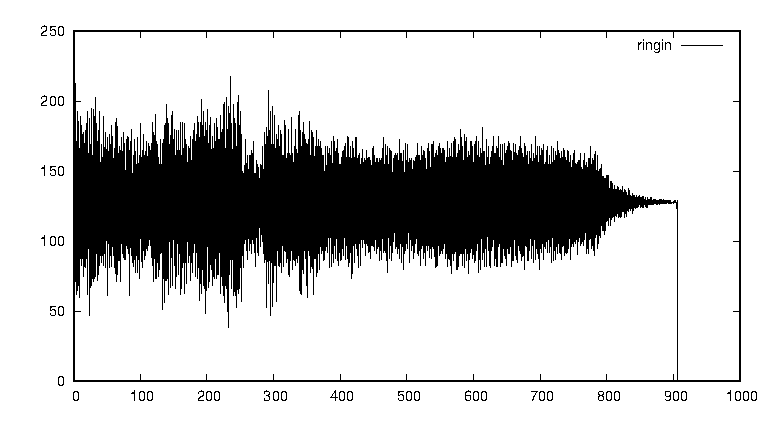
\includegraphics[width=7cm]{EPS/ringin.eps}
  \caption{ringin.wav}
  \label{ringin.wav}
\end{figure}

細かく振動することで波による上下差をなくし,比較的音のゆらぎの少ないファイルを作っているのだと思われる.
\subsubsection{ユーザが指定した周波数と振幅の正常波を1秒の長さだけ記録(録音)するプログラムを作成し,動作を確かめよ.}
ユーザが指定した周波数と振幅の正弦波を,モノラル音声で量子化ビット数8,サンプリング周波数11,025[Hz]で一秒の長さ記録するプログラムをソースコード\ref{rec-m8.c}に示す.
\begin{lstlisting}[caption=rec-m8.c,label=rec-m8.c]
#define BIAS 0x80
#define RIFF_SIZE 11061
#define FMT_SIZE 16
#define FORMAT_ID 1
#define SAMPLING_RATE 11025
#define CHANNEL_N 1
#define BLOCK_SIZE 1
#define Q_BIT 8
#define WAVE_SECOND 1
int data_size = SAMPLING_RATE * WAVE_SECOND;

void header_data(FILE *fp) {
  int riff_size = RIFF_SIZE;
  int fmt_size = FMT_SIZE;
  int format_id = FORMAT_ID;
  int channel_n = CHANNEL_N;
  int sampling_rate = SAMPLING_RATE;
  int block_size = BLOCK_SIZE;
  int q_bit = Q_BIT;
  int data_speed = sampling_rate * block_size;

  fwrite("RIFF", sizeof(char), 4, fp);
  fwrite(&riff_size, sizeof(int), 1, fp);
  fwrite("WAVE", sizeof(char), 4, fp);
  fwrite("fmt ", sizeof(char), 4, fp);
  fwrite(&fmt_size, sizeof(int), 1, fp);
  fwrite(&format_id, sizeof(short), 1, fp);
  fwrite(&channel_n, sizeof(short), 1, fp);
  fwrite(&sampling_rate, sizeof(int), 1, fp);
  fwrite(&data_speed, sizeof(int), 1, fp);
  fwrite(&block_size, sizeof(short), 1, fp);
  fwrite(&q_bit, sizeof(short), 1, fp);
  fwrite("data", sizeof(char), 4, fp);
  fwrite(&data_size, sizeof(int), 1, fp);
}

int main(int argc, char **argv) {
  int t;
  double amp, frq, rad, vin;
  unsigned char vout[SAMPLING_RATE];

  FILE *fp;
  if (argc < 4) {
    fprintf(stderr, "Usage: %s file page\n", argv[0]);
    return EXIT_FAILURE;
  }
  if ((fp = fopen(argv[3], "wb+")) == NULL) {
    fprintf(stderr, "File (%s) cannot open\n", argv[1]);
    return EXIT_FAILURE;
  }

  amp = atof(argv[1]);
  frq = atof(argv[2]);

  for (t = 0; t <= data_size; t++) {
    rad = t * (frq / SAMPLING_RATE) * 2 * PI;
    vin = amp * sin(rad) + BIAS;
    if (vin < 0) vin = 0;
    if (vin > 255) vin = 255;
    vout[t] = vin;
  }

  header_data(fp);
  fwrite(vout, sizeof(unsigned char), data_size, fp);
  fclose(fp);
  return EXIT_SUCCESS;
}
    \end{lstlisting}

これを用いて振幅100,周波数100[Hz]の正弦波を記録したWAVEファイルを作成した.再生してみて程よい重低音が聞こえたためこれでいいとおもわれるが,念のためソースコード\ref{wav2txt-m8.c}を使用して波形を観測してみた.その波形を図\ref{100f100_eps}に示す.
\begin{figure}[H]
  \centering
  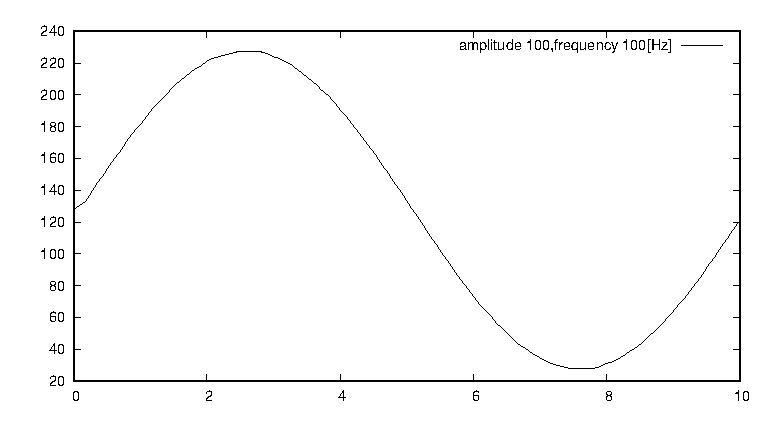
\includegraphics[width=7cm]{EPS/100f100.eps}
  \caption{WAVEファイルの波形}
  \label{100f100_eps}
\end{figure}

これを見る限り,しっかりと振幅100,周波数100[Hz]の正弦波が書きこまれていることがわかる.

仮にここでvoutの型をデータサイズが2Byte以上の型にしてしまうと,全く違う波形が生成されてしまうため,注意が必要である.
\section{あとがき}
\subsection{感想}
今回は波に関する実験を行ったが,色々な波形の作り方やWAVEファイルの構造や作り方など興味深い内容が多くあった.波について知ることはいろいろな場面で役に立つと思うので,今後もこれらについての理解を深めて行きたい.
\subsection{要望}
今回レポートを作成する際に気になった点として,gnuplotについての情報が従来の方法では手に入りづらい点が挙げられる.様々なエラーが発生するが,どこが悪いのかが分かりづらく関係するファイルもやや多いため,修正作業に時間がかかる.

ここについて情報が多く集まっているサイト等の記載があればもう少し楽になると考えられる.
\section*{参考文献}
\begin{enumerate}
  \item 令和4年度電子制御工学実験 $\cdot$ 4年前期テキスト
\end{enumerate}
\end{document}